\section{Flight Design for the Ground Transport}\label{sec:flight}
The path decides the reception map, so it is designed for River rather than for coverage.

\subsection{The delivery constraint}
Every cluster must be offered one complete copy of the query on its own cells, i.e., $Q\Tp=40.4$\,s of emission inside
the cluster. If the path through a cluster is shorter than $Q\Delta$, the UAV slows down, and if the minimum speed is not
enough it adds a loop of radius 63.7\,m at the CH. We call this adjustment \textsc{Fit}. Its consequence shapes the
design: a short path flown slowly costs the same in-cluster time as a long chord flown fast. What a planner can change
is therefore the transit between clusters, the visiting order, and how close the path comes to the cells that matter.

\subsection{\chord}
\chord{} flies one straight line through each cluster, through the CH, at the bearing of the longest in-cluster run; a
long chord gives a long \spine{} and hence many sources for River. The visiting order and directions minimise the mean
time at which critical cells are left behind, $\sum_c n_c\,t^{\mathrm{leave}}_c$ with $n_c$ the number of critical cells
of cluster $c$, by dynamic programming over (cluster, direction) with Dubins transits. The path is the same in every
A2G regime.

\subsection{\lmtour}
\lmtour{} replaces the longest chord by a path that is short and well placed (Algorithm~\ref{alg:lmtour}).

\emph{Step 1: tour through the cluster heads.} For each cluster and each of six bearings, a straight leg through the CH
is cut to its run over the cluster and passed through \textsc{Fit}; its cost is its delivery-feasible duration. The
legs, directions and order minimising $\sum_cW_c\,t^{\mathrm{leave}}_c$, with $W_c$ the total weight of the critical
cells of cluster $c$, are found by dynamic programming with Dubins transits. This is a DTSPN through discs of radius
$\xi$ around the CHs with
\begin{equation}
\xi=\min\bigl(\omega,\ \rho,\ R_{50}\bigr),
\end{equation}
so that a landmark within $\xi$ lies in the River band, the path can still turn there, and the landmark hears the UAV
directly; $\xi=255$, 255, 199 and 99\,m in the four regimes.

\emph{Step 2: bending towards landmarks.} Within each cluster the leg is bent, by smooth bumps of curvature at most
$1/\rho$ with the CH pinned, into the disc $B(k,\xi)$ of a critical cell $k$ whenever this lowers
\begin{equation}
\begin{aligned}
J_c=&\sum_{k\in K_c}w_k\,\mathrm{ready}_k+\Bigl(\sum_{k\in K_c}w_k\Bigr)t^{\mathrm{in}}_c\\
&+\theta\,W^{\mathrm{after}}_c\bigl(t^{\mathrm{in}}_c+\mathrm{dur}_c+t^{\mathrm{out}}_c\bigr),
\end{aligned}\label{eq:J}
\end{equation}
where $\mathrm{ready}_k=\min\{\mathrm{own}_k,\ \mathrm{dur}_c+\widehat T_{\mathrm{River}}(k)\}$ is the earlier of the cell
decoding by itself along the pass and River completing it, $\mathrm{dur}_c$ is the pass duration after \textsc{Fit},
$t^{\mathrm{in}}_c,t^{\mathrm{out}}_c$ are the Dubins transits to the neighbouring passes and $W^{\mathrm{after}}_c$ is
the weight of the clusters flown later. $\widehat T_{\mathrm{River}}$ is the surrogate \eqref{eq:surrogate}, evaluated on
the River plan of the candidate path. Bending stops when no candidate lowers $J_c$.

\begin{algorithm}[t]\caption{\lmtour}\label{alg:lmtour}
\begin{algorithmic}[1]\footnotesize
\REQUIRE clusters with CH and critical cells, weights $w$, $\xi$, $\theta$
\FORALL{cluster $c$, bearing $b\in\{0^\circ,30^\circ,\dots,150^\circ\}$}
\STATE $\ell_{c,b}\leftarrow$ line through $\mathrm{CH}_c$ at bearing $b$, cut to its run over $c$; cost
$\leftarrow$ duration of \textsc{Fit}$(\ell_{c,b})$
\ENDFOR
\STATE (legs, directions, order) $\leftarrow\argmin\sum_cW_c\,t^{\mathrm{leave}}_c$ with Dubins transits
\FORALL{cluster $c$}
\STATE $\mathit{cur}\leftarrow$ leg of $c$; $\mathit{pulls}\leftarrow\emptyset$
\REPEAT
\FORALL{$k\in K_c\setminus\mathit{pulls}$ with $w_k\ge w_{\min}$ farther than $\xi$ from $\mathit{cur}$}
\STATE $\gamma_k\leftarrow$ leg bent into $B(k',\xi)$ for $k'\in\mathit{pulls}\cup\{k\}$; keep it if it crosses $c$ once
\STATE evaluate $J_c(\gamma_k)$: \textsc{Fit}, River plan, surrogate \eqref{eq:surrogate}
\ENDFOR
\STATE $k^\star\leftarrow\argmin_kJ_c(\gamma_k)$; \textbf{if} $J_c(\gamma_{k^\star})<J_c(\mathit{cur})$ \textbf{then}
$\mathit{pulls}\leftarrow\mathit{pulls}\cup\{k^\star\}$, $\mathit{cur}\leftarrow\gamma_{k^\star}$
\UNTIL{no improvement}
\ENDFOR
\RETURN the passes and their River plans
\end{algorithmic}
\end{algorithm}

\textbf{Surrogate.} Running ns-3 for every candidate is infeasible, so the BS uses \eqref{eq:surrogate}, fitted on the
completion times of 812 critical cells in ns-3. Its three features are computable before take-off from the path, the
deployment and the channel regime; the lack predicted by the reception model matches the lack observed in ns-3 (mean
2200 against 2183 packets). At mission level the predicted difference between \lmtour{} and \chord{} is within 10\,s of
the one later measured in ns-3 ($-38$, $-93$, $-89$, $-90$\,s predicted against $-38$, $-83$, $-84$, $-90$\,s measured on the
8-cluster map), which is what the planner needs: a ranking of paths.

\textbf{What the two steps contribute.} Because of the delivery constraint, the tour of Step~1 already yields most of the
gain over \chord: the in-cluster time stays near 40\,s while the transits shrink. Bending adds 7--22\,s on the
8-cluster map and saturates after one or two pulls per cluster, since pulling the path towards a cell changes that
cell's hop count and part of its lack but hardly the total lack of the cluster, which dominates \eqref{eq:surrogate}.

\begin{figure*}[t]\centering
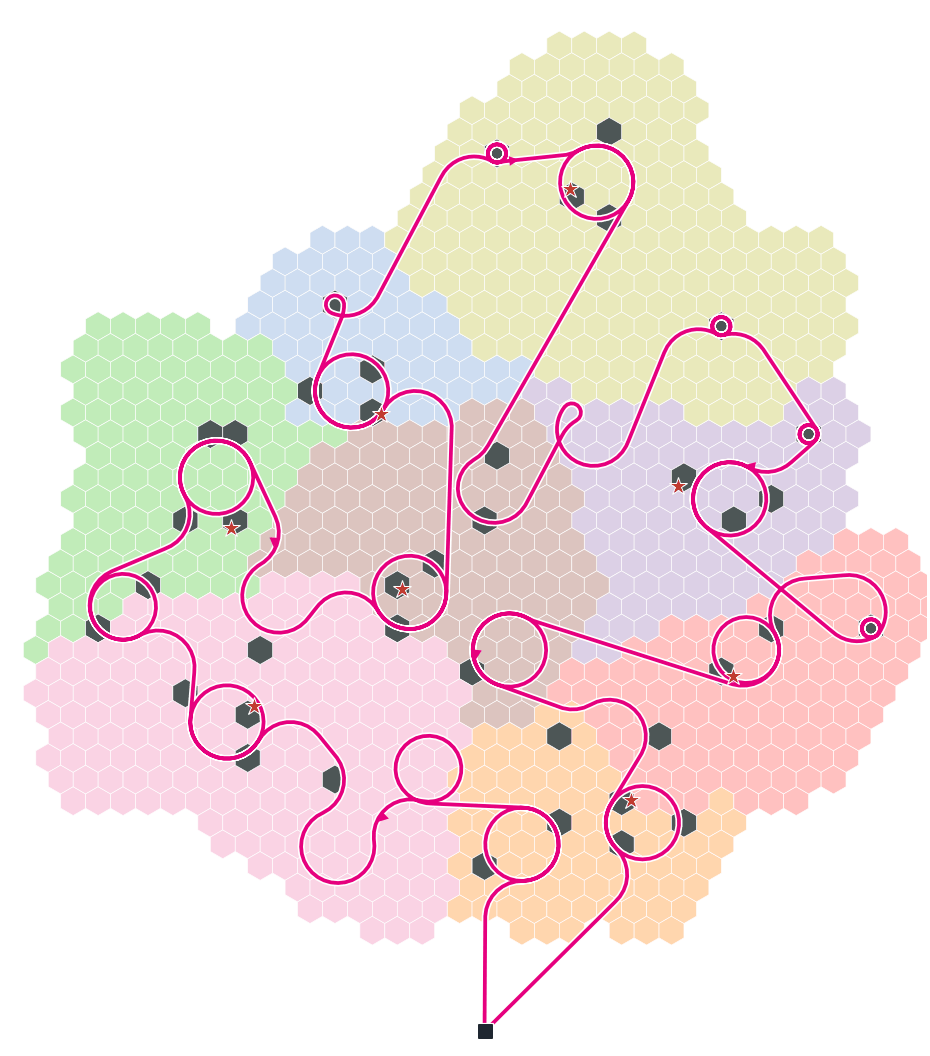
\includegraphics[width=0.21\textwidth]{c4-phase1-k8-s1-r500-fc-dtspn-mono.png}\hfill
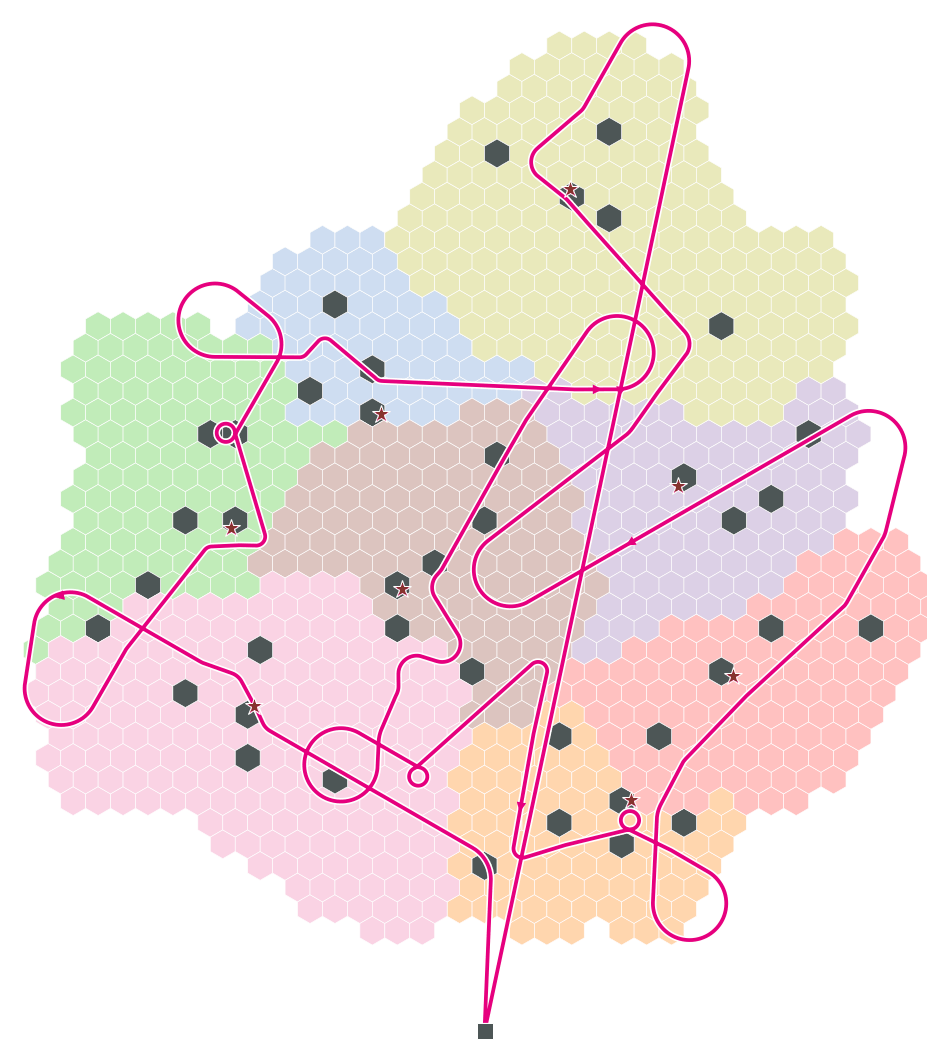
\includegraphics[width=0.21\textwidth]{c4-phase1-k8-s1-r500-dtspn-river-mono.png}\hfill
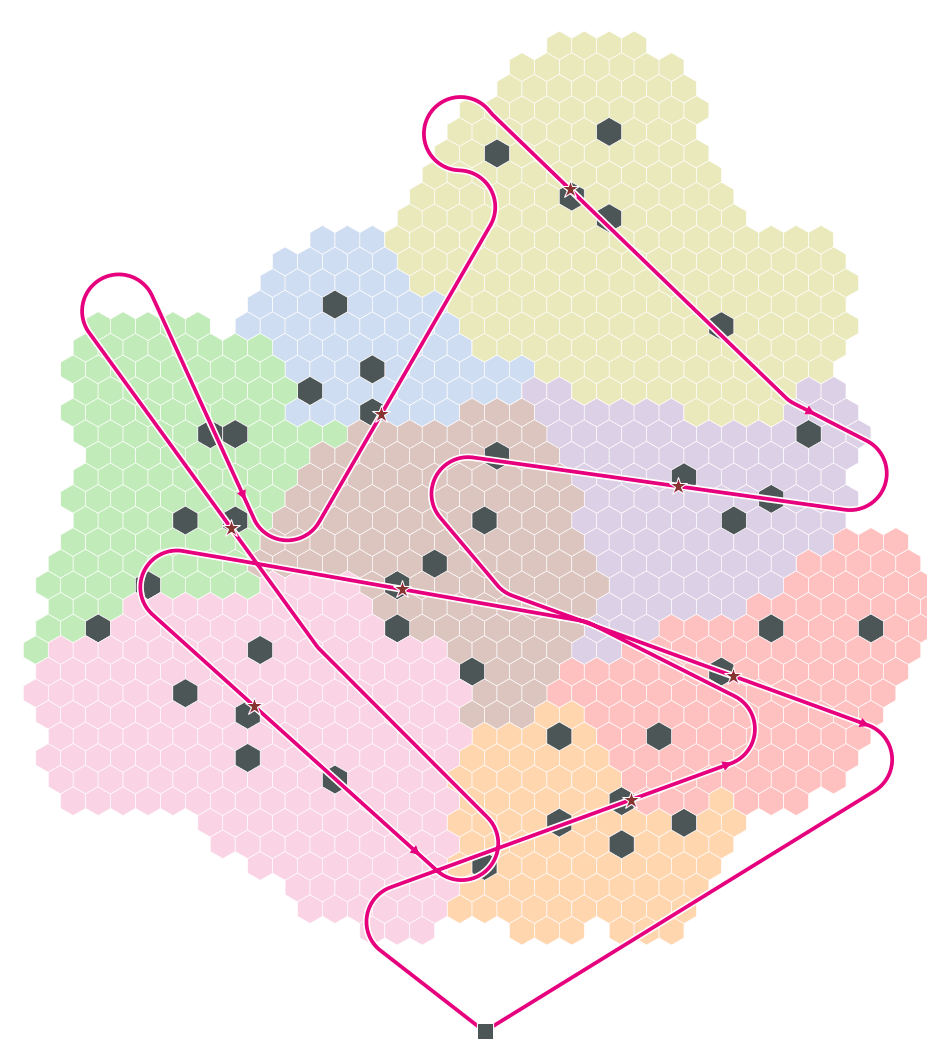
\includegraphics[width=0.21\textwidth]{c4-phase1-k8-s1-r500-chord-mono.png}\hfill
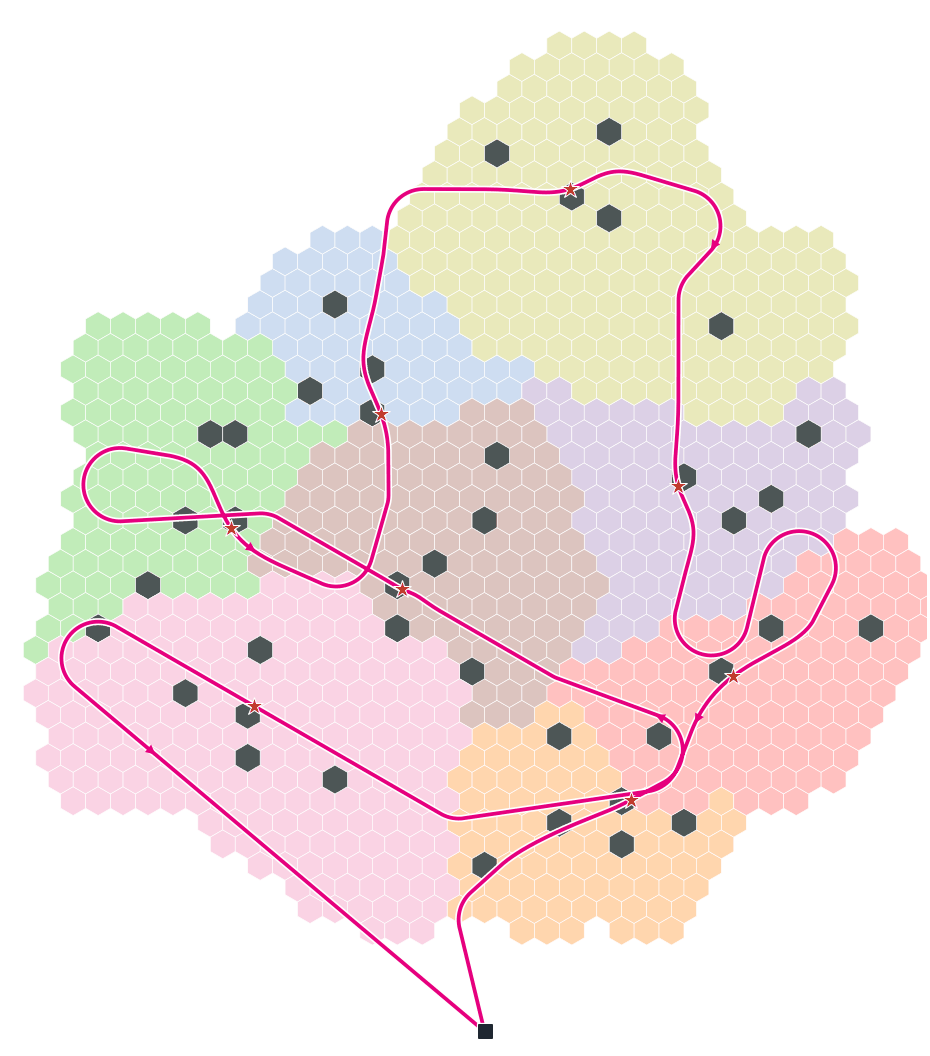
\includegraphics[width=0.21\textwidth]{c4-phase1-k8-s1-r500-lmtour-mono.png}
\caption{Team-1 paths on the 8-cluster map at $R_{50}=498$\,m. From left: FC+DTSP-N (58.7\,km, 1320\,s, orbits around
groups of critical cells), DTSP-N+River (46.6\,km, 1066\,s, into the disc of every critical cell), \chord{}+River
(38.6\,km, 784\,s) and \lmtour{}+River (30.8\,km, 699\,s; small loops are the \textsc{Fit} loops).}\label{fig:paths}
\end{figure*}
